\section{Estimation of $\langle$\#ori$\rangle$ / $\langle$\#ter$\rangle$ and $\langle$\#ori$\rangle$.}

\textit{E. coli} shows robust scaling of cell size with average the number of
origins $\langle$\#ori$\rangle$ per cell \citep{si2017}. Since protein makes up
a  majority of the cell's dry mass, the change is cell size is also a reflection
of the changes in proteomic composition and total abundance across growth
conditions. Given the potential constraints on rRNA synthesis with
$\langle$\#ori$\rangle$ (limited by the effective number of rRNA gene copies),
it is important to consider how protein copy numbers vary with the state of
chromosomal replication. This is particularly true  when trying to connect the
dependence of growth rate on ribosomal fraction with  particular mechanism the
cell employs to vary ribosomal synthesis.  As considered in the main text, it is
becoming increasingly apparent that regulation through the secondary messengers
(p)ppGpp acts to throttle back DNA replication and ribosomal activity in poorer
nutrient conditions.  In this context, both $\langle$\#ori$\rangle$, as well as
the $\langle$\#ori$\rangle$ / $\langle$\#ter$\rangle$ ratio become important
parameters to consider and keep tract of. An increase in $\langle$\#ori$\rangle$
/ $\langle$\# ter$\rangle$ ratio  in particular, causes a relatively higher gene
dosage in rRNA and r-protein genes due to skew in genes near the origin, where
the majority of these are located

In the main text we estimated the change in $\langle$\#ori$\rangle$ with growth
rate using the nutrient-limited wild-type cell data from \cite{si2017}. We
consider their measurements of DNA replication time ($t_{C}$, 'C' period of
cell division), total cell cycle time ($t_{cyc}$, 'C' + 'D' period of cell
division), and doubling time $\tau$ from wild-type \textit{E. coli} growing
across a range of growth conditions. Here we show how we  esimate this
parameter, as well as the $\langle$\#ori$\rangle$ / $\langle$\# ter$\rangle$
ratio from their data.  We begin by considering $\langle$\#ori$\rangle$. If the
cell cycle time takes longer  than the time of cell division, the cell will need
to initiate DNA replication  more often than its rate of division, $2^{\lambda
t} = 2^{ln(2) \cdot t/ \tau}$ to maintain steady-state growth. Cells will need
to do this in proportion to the ratio $\lambda_{cyc} / \lambda =  t_{cyc}/\tau$,
and the number of origins per cell (on average) is then given by $2^{t_{cyc}/
\tau}$.   The average number of termini will in contrast depend on the lag time
between  DNA replication and cell division, $t_{D}$, with
$\langle$\#ori$\rangle$ / $\langle$\# ter$\rangle$ ratio = $2^{t_{cyc}/ \tau -
t_{D}/ \tau} =  2^{t_{C}/ \tau}$.

In Figure \ref{fig:Si_Cm}(A) and (B) we plot the measured $t_{C}$ and $t_{cyc}$
values versus the doubling time from \cite{si2017}. The authors estimated
$t_{C}$ by marker frequency analysis using qPCR, while  $t_{cyc} = t_{C} +
t_{D}$ were inferred from $t_{C}$ and $\tau$. In the plots we see that both
$t_{C}$ and $t_{cyc}$ reach a minimum  at around 40 and 75 minutes,
respectively. For a C period of 40 minutes, this would correspond to a maximum
rate of elongation of about 1,000 bp/sec. Since we lacked a specific model to
describe how each of these parameters vary with growth condition, we assumed
that they were linearly dependent on the doubling time. For each parameter,
$t_{C}$ and $t_{cyc}$, we split them up into two domains corresponding to poorer
nutrient conditions and rich nutrient conditions (cut off at $\tau \approx$ 40
minutes where chromosomal replication becomes nearly constant). The fit lines
are shown as solid black lines. In Figure \ref{fig:Si_Cm}(C) and (D) we also
show $t_{C}$ and $t_{cyc}$ as a function of growth rate $\lambda$ along with our
piecewise linear fits, which match the plots in the main text.


\begin{figure}
    \begin{fullwidth}
        \centering{
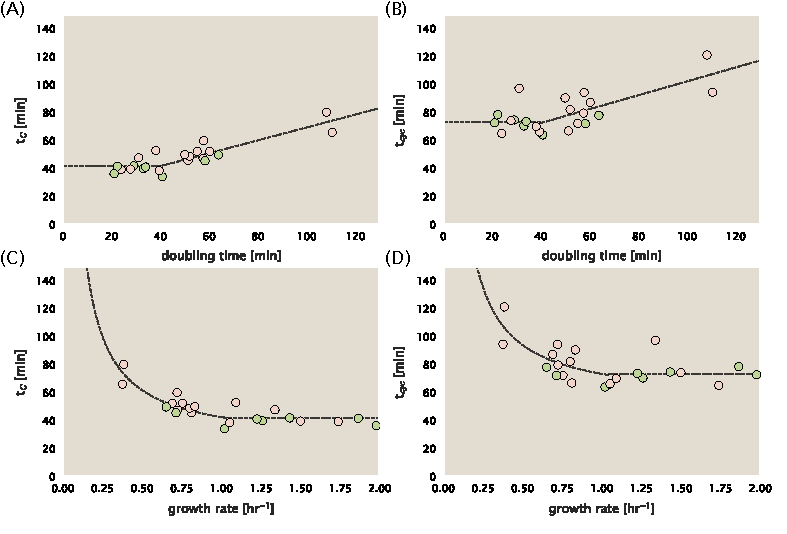
\includegraphics{SI_figs/supplemental_ori_ter.pdf} \caption{\textbf{Estimation of
    $\langle$\#ori$\rangle$ / $\langle$\# ter$\rangle$ and
    $\langle$\#ori$\rangle$ using data from Si \textit{et al.} (2017).} (A) and
    (B) plot the reported $t_{C}$ and $t_{cyc}$ as a function  of cell doubling
    time $\tau$, respectively. The dashed lines show a piecewise fit to  the
    data. For short doubling times (rich media), $t_{C}$ and $t_{cyc}$ are
    assumed  constant. At the transition, taken to occur at 40 minutes, the
    dashed line corresponds  to an assumed proportional increase in each
    parameter as a function of the doubling time. (C) and (D) plot the same data
    as in (A) and (B), but as a function of growth rate, given by $\lambda = ln(2)/\tau$.}
\label{fig:Si_tC_tcyc} }
\end{fullwidth}
\end{figure}

\section{Calculation of active ribosomal fraction.}

In the main text we used the active ribosomal fraction $f_a$ that was reported
in the work of \cite{dai2016} to estimate the active ribosomal mass fraction
$\Phi_R \times f_a$ across growth conditions. We lacked any specific model to
consider how  $f_a$ should vary with growth rate, and instead find that the data
is well-approximated by fitting to an exponential curve ($f_a$ = -0.889 $e^{4.6
\cdot \lambda}$ + 0.922; dashed line in inset of \FIG{ribosome_limit}(C)). We
use this function to estimate $f_a$ for each of the data points shown in
\FIG{ribosome_limit}(C).


% of actively translating ribosomes across
% the different datasets available based on the growth-rate dependent measurements from the work
% of \citep{dai2016}. Here we provide additional details on how $f_a$ was initially determined,
% and how we have used it to estimate the active ribosomal fraction for each data set.

% In the work of \citep{dai2016}, the authors independently measured the
% translation rate, ribosomal abundance (via the total RNA-to-protein ratio), and
% growth rate $\lambda$ across a vast range of growth conditions (growth rates spanning ~ 0
% - 2 h$^{-1}$). By requirements of mass balance, and an assumption that cells are doubling their
% proteome with each cell division under steady-state growth, we expect,
%
% \begin{equation}
%   r_t \cdot R  \lambda \cdot N_{aa}.
% \end{equation}
% $r_t$ is the translation elongation rate, $R$ is the number of ribosomes, and $N_{aa}$ is the number of peptide bonds that must be formed to double the cell's protein mass. An important observation from the work of \citep{dai2016} was that their measured translation rates and ribosomal abundance were incompatible with this expectation. This was particularly true at slow growth (below about 0.7 h$^{-1}$). The explanation arrived at by the authors is that cells are regulating the fraction of ribosomes that are translating. As further support for this idea, sublethal concentrations of chloramphenicol caused a further decrease in the apparent
% fraction of actively translating ribosomes.
%
% In Figure X we show the reported values of $f_a$ as a function of growth rate
%
% in order to maintain
%
%
%  \cdot R \cdot f_a$ $N_{aa}This corresponds to Equation 3 in the main text, where the
%
% estimate the fraction


% \section{Average protein expression across the chromosome.}
%
% In Figure 7(B) of the main text we plotted the average protein copy number along
% \textit{E. coli}'s chromosome using a boxcar averaging (i.e. running average)
% window of 0.5 Mb. This means that at each position on the chromosome, proteins
% with a transcription start site that were +/- 0.25 Mb from that position
% were  included in the calculated average. For \textit{E. coli},
% position 0 bp does not correspond the location of the origin and we  keep to
% this convention, using the reported positional information from EcoCyc. Since
% the chromosome is circular, when calculating the  average at positions  near the
% end positions (i.e. near either 0 bp or 4.6 Mb) we include the copy numbers
% on opposing ends.  For example, calculating the average for position 0 bp would
% include the range from 4.1 Mb to 0.25 Mb).  Here we provide some additional
% analysis to show how the absolute copy numbers compare across growth conditions,
% as well as the effect of the specific averaging window size.
%
% In the main text we centered each data set according to the mean average in order
% to  compare the relative changes in copy number along the length of the
% chromosome in each data set. In reality, there is also a correlation between the
% total genomic content and protein copy number, which increases at faster growth.
% This is shown in Figure \ref{fig:supplemental_boxcar_1}(A), where we plot the boxcar average from each
% growth condition without rescaling each about their mean values.
%
% \begin{figure}
%     \begin{fullwidth}
%         \centering{
% 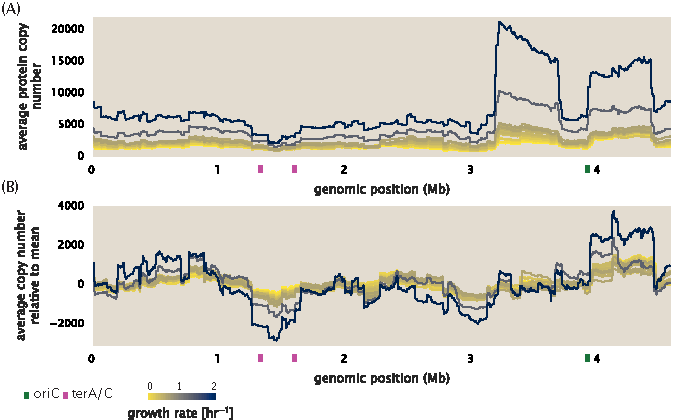
\includegraphics{SI_figs/supplemental_boxcar1.pdf} \caption{\textbf{Position-dependent protein expression at different growth rates.} (A) Protein copy number is reported along the length of the chromosome using a boxcar averaging, with window size of 0.5 Mb.
%   (B)The boxcar average protein copy number, shifted relative to the mean value for each
%   growth conditions, is show for a window size of 0.5 Mb. In this plot, all ribosomal
%   proteins and elongation factor EF-Tu were excluded in the analysis.}
% \label{fig:supplemental_boxcar_1} }
% \end{fullwidth}
% \end{figure}
%
% One of the challenges in interpreting this analysis is that the protein copy
% numbers for a small subset of proteins vary dramatically as a function of growth
% rate. This is particularly true for ribosomal proteins. In order to check
% whether the result is due simply due to the change in ribosomal copy number, we
% repeated the analysis with all ribosome proteins, and the translation elongation
% factor EF-Tu removed (Figure \ref{fig:supplemental_boxcar_1}(B)). Indeed we still
% see a skew in  protein abundance, with higher overall expression at the origin.
%
% The other important parameter in this analysis is the size of the averaging
% window, which we took at 0.5 Mb. In Figure \ref{fig:supplemental_boxcar_2} we show
% the  results when using averaging window sizes of 0.05 Mb, 0.25 Mb, 0.5 Mb, 1
% Mb, and 2 Mb. Aside from the smallest window size of 0.05 Mb, the analysis seems
% to show a similar result, with proteins near the origin showing highest
% expression. For the window size of  0.05 Mb, the copy numbers become much
% noisier due to the large differences in protein copy number  that are observed
% irrespective of the specific growth rate.
%
% \begin{figure}
%     \begin{fullwidth}
%         \centering{
% 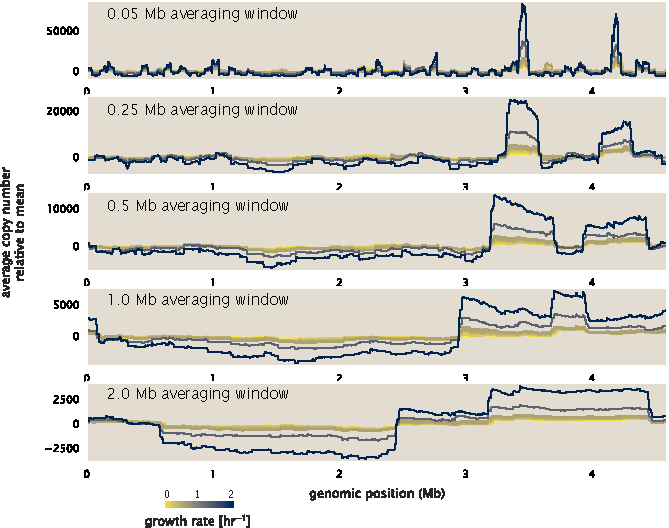
\includegraphics{SI_figs/supplemental_boxcar2.pdf} \caption{\textbf{Position-dependent protein expression at different growth rates.} (A) Protein copy number is reported along the length of the chromosome using a boxcar averaging. Here we consider different averaging window sizes:
% 0.05 Mb, 0.25 Mb, 0.5 Mb, 1.0 Mb, and 2 Mb. }
% \label{fig:supplemental_boxcar_2} }
% \end{fullwidth}
% \end{figure}


%
% \section{Hypothesis for increase in ribosomal abundance in the presence of chloramphenicol.}
%
% In the main text we note that the observed increase in ribosomal abundance  upon
% addition of non-lethal concentrations of chloramphenicol may in part  be a
% consequence of limiting rRNA production. Specifically, the proposal assumes that
% RNA polymerase are producing rRNA at their maximal rate (i.e. maximal packing of
% RNA polymerase on each rRNA operon). By sequestering ribosomes there will be a
% decrease in protein synthesis rate (i.e. lower $r_t \cdot R$) and a
% corresponding increase in doubling time. Qualitatively then, we may then expect
% that that more rRNA (and therefore more ribosomes) may be produced for a
% specific growth condition and longer doubling times  Figure
% \ref{fig:Si_Cm}(A).
%
% Here we consider data from Si \textit{et al.} (2017) where cells were grown in
% the presence of sub-lethal levels of chloramphenicol. In Figure \ref{fig:Si_Cm}(B) we
% plot measured RNA-to-protein ratios as a function of $\langle$\#ori$\rangle$ /
% $\langle$\# ter$\rangle$ (calculated using their reported values of $\tau_C$ and
% $\tau$). While the data is relatively noisy, we do see that
% increasing concentrations of chloramphenicol is associated with an increased
% RNA-to-protein ratios and this appears roughly independent of the particular
% $\langle$\#ori$\rangle$ / $\langle$\# ter$\rangle$ ratio.
%
% One challenge in interpreting the data is that the $\langle$\#ori$\rangle$ /
% $\langle$\# ter$\rangle$ ratio for a specific growth condition tends to decrease
% with increasing concentrations of chloramphenicol (indicated by marker type).
% Since the $\langle$\#ori$\rangle$ / $\langle$\# ter$\rangle$ ratio is defined by
% the ratio $\tau_C$/ $\tau$, this is likely a reflection of chloramphenicol
% slowing down protein production relative to the rate of DNA replication (though,
% both $\tau_C$ and $\tau$ increase with added chloramphenicol).
%
% Lastly, using the reported cell size data that was also available, we also
% consider how total ribosome copy number varies with growth condition and
% chloramphenicol. Here, as a first approaximation we assume that the total
% protein per cell will is proportional to cell size (with total protein $\approx$
% cell volume x 1.1 g/ml x 30\% dry mass x 55\% protein). We then estimate the
% number of ribosomes by multiplying the protein mass by our estimate of the
% ribosomal fraction.  Consistent with the apparent generality in how growth
% relates to cell size (size $\propto$ $\langle$\#ori$\rangle$) \citep{si2017},
% the number of ribosomes per cell collapse  onto a roughly linear trend with
% respect to the  $\langle$\#ori$\rangle$ (Figure \ref{fig:Si_Cm}(C)).
%
% That each of the chloramphenicol curves do not collapse onto a single line when
% normalized relative to $\langle$\#ori$\rangle$ (Figure \ref{fig:Si_Cm}(D))
% may be a reflection of biosynthetic rates increasing overall in richer media.
% For protein translation specifically, the rate of translation increases in both
% nutrient-limitation \citep{scott2010}, and with increasing concentrations of
% chloramphenicol \citep{dai2016} for poorer media (up to maximum of about 17 aa
% per second). It may be that other processes, and production of rRNA in
% particular may also slow down in poorer media.
%
% \begin{figure}
%     \begin{fullwidth}
%         \centering{
% 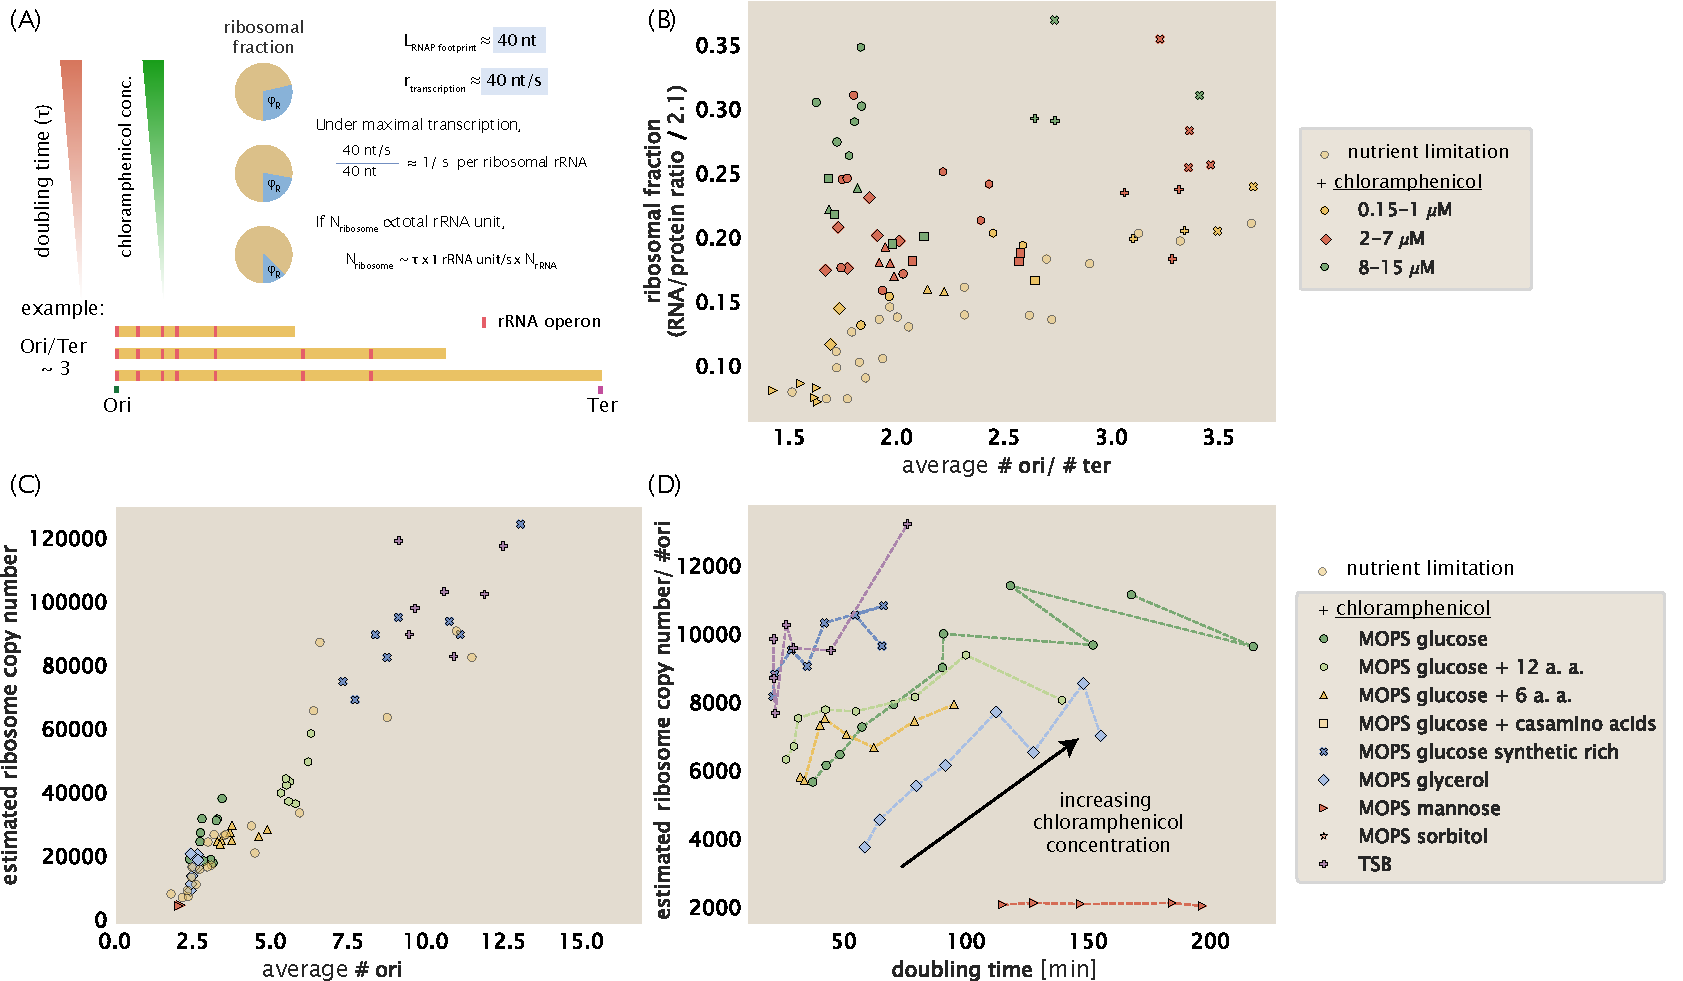
\includegraphics[width=1.2\textwidth]{SI_figs/supplemental_Si_Cm.pdf} \caption{\textbf{Potential effect of
%     chloramphenicol on ribosomal abundance of if rRNA production is limiting.}
%     (A) Schematic of proposed change in ribosomal abundance upon addition of non-lethal
%     does of chloramphenicol. We consider, for example, a $\langle$\#ori$\rangle$ / $\langle$\#ter$\rangle$ ratio of ~ 3, which reflects an effective chromosome whose gene dosage is biased more so to regions near the origin. If ribosome production is limited by
%     rRNA production in particular, then sequestering ribosomes will slow down
%     cell doubling and provide addition time for more rRNA to be made.
%     (B) Estimated ribosomal fraction ($\approx$ RNA/protein ratio x 2.1 \cite{dai2016}) at
%     as a function of measured $\langle$\#ori$\rangle$ / $\langle$\# ter$\rangle$ ratio. Data is
%     split into 'nutrient-limited' growth (pale yellow), low chloramphenicol concentration (yellow, 0.15 - 1 $\mu$M), medium chloramphenicol concentration (red, 2 - 7 $\mu$M), and
%     high chloramphenicol concentration (red, 8 - 15 $\mu$M). Marker type corresponds to
%     the growth media as indicated in part (C).
%     (C) Scaling of estimated ribosomal copy number with $\langle$\#ori$\rangle$, showing that
%     cells still scale their total protein in accord with apparent growth law \citep{si2017}
%     irrespective of presence of chloramphenicol.
%     (D) Estimated ribosomal copy number normalized by $\langle$\#ori$\rangle$. Data shows
%     a media-specific increase in ribosomal abundance per origin with longer doubling times.
%     All data is from \citep{si2017}, and show that average values from each growth condition and chloramphenicol concentration (including data from both strains, MG1655 and NCM3722).}
% \label{fig:Si_Cm} }
% \end{fullwidth}
% \end{figure}
%
%
